\subsection{Berechnung der Fouriertransformation mittels FFT}
Die Mathematiker Cooley und Tukey haben einen Algorithmus entwickelt, mit dem sich die Fouriertransformation mit vergleichsweise wenig Multiplikationen
und somit deutlich schneller als bei der allgemeinen \gls{dft} berechnen lässt.

Es ist erforderlich, dass hierfür die Werte im Eingangsvektor in umgekehrter Bitrehenfolge getauscht. Dies geschieht nach dem Muster, dass die Indizes der Eingangswerte wie
üblich bei 0 beginnend binär dargestellt werden. Nun wird die Reihenfolge der Bits getauscht. Auf diese Weise tauschen bei einem 8-Bit Vektor die
Werte 2 und 5 sowie 4 und 7 ihre Position.


\begin{figure}[htbp]
 \centering
 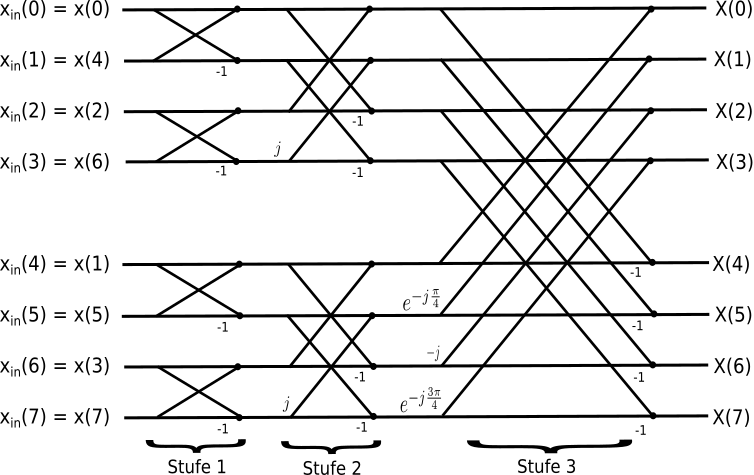
\includegraphics[width=0.7\textwidth]{img/Butterfly.png}
 \caption{8x8 Butterfly}
 \label{pic:Butterfly}
\end{figure}
